\documentclass{beamer}

\usepackage{predavanja}
\usepackage{amsfonts}  % Dodajanje paketa za matematične pisave (npr. \mathbb)
\usepackage{tikz}      % Za risanje diagramov znotraj dokumenta
\usetikzlibrary{math}  % Uporaba dodatne knjižnice za matematične operacije v TikZ-u

\usepackage{pgfplots}  % Za risanje grafov znotraj dokumenta
\usepgfplotslibrary{external}  % Omogoči zunanjo obdelavo grafov za hitrejše kompiliranje

\usepackage{array}  % Omogoči napredno delo s tabelami

\theoremstyle{definition}
\newtheorem{definicija}{Definicija}  % Definicija za okolje definicija
\newtheorem{vaja}{Vaja}
\newtheorem{izrek}{Izrek}  % Definicija za okolje izrek

% Definicija okrajšav za cela, realna in kompleksna števila
\newcommand{\ZZ}{\mathbb{Z}}  % Cela števila
\newcommand{\RR}{\mathbb{R}}  % Realna števila
\newcommand{\CC}{\mathbb{C}}  % Kompleksna števila

\begin{document}

\title{Matematični izrazi in uporaba paketa \texttt{beamer}}
\subtitle{\emph{Matematičnih} nalog ni treba reševati!}
\institute{Fakulteta za matematiko in fiziko}
\date{}  % Dodajanje praznega datuma

% Prva stran z naslovom
\frame{\titlepage}

% Kratek pregled vsebine
\begin{frame}
    \frametitle{Kratek pregled}
    \tableofcontents %[pausesections]
\end{frame}

% Sekcija 1 - Paket beamer
\section{Paket \texttt{beamer}}
%  Naslov prosojnice lahko naredimo tudi z dodatnim parametrom okolja `frame`.
\begin{frame}{Posebnosti prosojnic}
	    Za prosojnice je značilna uporaba okolja \texttt{frame},
	    s katerim definiramo posamezno prosojnico, \pause
	    postopno odkrivanje prosojnic, \pause
	    ter nekateri drugi ukazi, ki jih najdemo v paketu \texttt{beamer}. \pause
	\begin{exampleblock}{Primer}
		Verjetno ste že opazili, da za naslovno prosojnico niste uporabili
		ukaza \texttt{maketitle}, ampak ukaz \texttt{titlepage}.
	\end{exampleblock}	
\end{frame}


\begin{frame}{Poudarjeni bloki}

	\begin{block}{Opomba}
		Okolja za poudarjene bloke so \texttt{block}, \texttt{exampleblock} in \texttt{alertblock}.
	\end{block}	
	    
    \begin{alertblock}{Pozor!}
		Začetek poudarjenega bloka (ukaz \texttt{begin}) vedno sprejme 
		dva parametra: okolje in naslov bloka.
		Drugi parameter (za naslov) je lahko prazen. 
	\end{alertblock}
		
\end{frame}


\begin{frame}{Tudi v predstavitvah lahko pišemo izreke in dokaze}

	\begin{izrek}
	   Praštevil je neskončno mnogo.
	\end{izrek}

	\begin{proof}
	   Denimo, da je praštevil končno mnogo.
	   	
	   \begin{itemize}[<+->]
		  \item Naj bo $p$ \alert<4>{največje} praštevilo.
		  \item Naj bo $q$ produkt števil $1$, $2$, \ldots, $p$.
		  \item Število $q+1$ ni deljivo z nobenim praštevilom, torej je $q+1$ praštevilo.
		  \item To je protislovje, saj je $q+1>p$. \qedhere
	   \end{itemize}

	\end{proof}

 \end{frame}
 

% Sekcija 2 - Paketa amsmath in amsfonts
\section{Paketa \texttt{amsmath} in \texttt{amsfonts}}
\begin{frame}{Matrike}
	
	Izračunajte determinanto
	\[
	\begin{vmatrix}
	     -1 & 4 & 4 & -2 \\
		 1 & 4 & 5 & -1 \\
		 1 & 4 & -2 & 2 \\
		 3 & 8 & 4 & 3 \\
	\end{vmatrix}
	\]
	V pomoč naj vam bo Overleaf dokumentacija o matrikah:
	
	\href{https://www.overleaf.com/learn/latex/Matrices}{\beamergotobutton{Matrices}}

\end{frame}


\begin{frame}{Okolje \texttt{align} in \texttt{align*}}

    Dokaži \emph{binomsko formulo}: za vsaki realni števili $a$ in $b$ in za vsako naravno število $n$ velja
		   
	\begin{align*}
        (a+b)^n & = \only<1>{\ldots} \onslide<2,3>{(a+b)(a+b)\dots(a+b)} \\
	\onslide<3>{& = a^n + na^{n-1} b + \dots + \binom{n}{k} a^{n-k} b^k + \dots + n a b^{n-1} + b^n} \\       
	            & = \sum_{k=0}^n \binom{n}{k} a^{n-k} b^k		
	\end{align*}
\end{frame}


\begin{frame}{Še ena uporaba okolja \texttt{align*}}
	
Nariši grafe funkcij:
	\begin{align*}	
	y &= x^2 - 3|x| + 2 &   y &= 3 \sin(\pi+x) - 2 \\
	y &= \log_2(x-2) + 3 &   y &= 2 \sqrt{x^2+15} + 6 \\
	y &= 2^{x-3} + 1    &   y &= \cos(x-3) + \sin^2(x+1) 
    \end{align*}
\end{frame}


\begin{frame}{Okolje \texttt{multline}}
	
	Poišči vse rešitve enačbe
	\begin{multline}
	(1+x+x^2) \cdot (1+x+x^2+x^3+\ldots+x^9+x^{10}) = \\
	= (1+x+x^2+x^3+x^4+x^5+x^6)^2.	
	\end{multline}
\end{frame}


\begin{frame}{Okolje \texttt{cases}}
	
	Dana je funkcija
	\[
	f(x,y) = 
	\begin{cases}
	\frac{3x^2y-y^3}{x^2+y^2};&  (x,y) \neq (0,0), \\
	a; &                         (x,y) = (0,0).
	\end{cases}
	\]

	\begin{itemize} 
	\item Določi $a$, tako da izračunaš limito \( \lim_{(x,y)\to(0,0)} f(x). \)
	\item Izračunaj parcialna odvoda $f_x(x,y)$ in $f_y(x,y)$.
	\end{itemize}
\end{frame}


% Sekcija 3 - Matematične vsebine (Analiza, logika, množice)
\section[Matematika, 1. del\\\large{Analiza, logika, množice}]{Matematika, 1. del}
\begin{frame}{Logika in množice}
	\begin{enumerate}
		\item
		Poišči preneksno obliko formule \(
\exists x \colon P(x) \land \forall x \colon Q(x) \Rightarrow \forall x \colon R(x)
\)
.
		\item 
		Definiramo množici \($A$ = \lbrack 2,5 \rbrack\) in \($B$ = \lbrace 0,1,2,3,4\ldots \rbrace\).
		V ravnino nariši:
		\begin{enumerate}
		   \item \(A \cap B \times \emptyset\)
		   \item \((A \cup B)^c \times \mathbb{R}\)
		\end{enumerate}
		\item
		Dokaži:
		\begin{itemize}
			\item \((A \Rightarrow B) \sim (\neg B \Rightarrow \neg A)\)
			\item \(\neg (A \lor B) \sim \neg A \land \neg B \)
		\end{itemize}
	\end{enumerate}
\end{frame}

\begin{frame}{Analiza}
	\begin{enumerate}
		\item
		Pokaži, da je funkcija \(x \mapsto \sqrt{x}\) enakomerno zvezna na \([0,\infty)\).
		\item 
		Katero krivuljo določa sledeč parametričen zapis?
		% Spodaj si pomagajte z dokumentacijo o razmikih v matematičnem načinu.
		% https://www.overleaf.com/learn/latex/Spacing_in_math_mode
		$$
		   x(t) = a \cos t, \quad  
		   y(t) = b \sin t, \quad 
		   t \in [0, 2 \pi]
		$$ 
		\item
		Pokaži, da ima \( f(x) = 3x + sin(2x) \) inverzno funkcijo in izračunaj \((f^-1)'(3\pi)\).
		
		\item
		Izračunaj integral 
		% V rešitvah smo spodnji integral zapisali v vrstičnem načinu,
		% ampak v prikaznem slogu. To naredite tako, da v matematičnem načinu najprej
		% uporabite ukaz displaystyle.
		% Pred dx je presledek: pravi ukaz je \,
		\(\int \frac{2+\sqrt{x+1}}{(x+1)^2-\sqrt{x+1}} dx\)
		%  
		\item 
		Naj bo $g$ zvezna funkcija. Ali posplošeni integral 
		\(\int_{0}^{1} \frac{g(x)}{x^2} dx\)
		konvergira ali divergira? Utemelji.
	\end{enumerate}
\end{frame}

\begin{frame}{Kompleksna števila}
	\begin{enumerate}
		\item
		Naj bo $z$ kompleksno število, $z \ne 1$ in $|z| = 1$.
		Dokaži, da je število \( i \, \frac{z+1}{z-1} \) realno.
		\item
		Poenostavi izraz:
		\[\frac{\frac{3 + i}{2 - 2i} + \frac{7i}{1 - i}}{1 + \frac{i - 1}{4} - \frac{5}{2 - 3i}}\]
	\end{enumerate}
\end{frame}

% Sekcija 4 - Stolpci in slike
\section{Stolpci in slike}
\begin{frame}{Konstrukcija pravokotnice na premico $p$ skozi točko $T$}

		  \begin{itemize}
			 \item Dani sta premica $p$ in točka $T$.
			 \item Nariši lok $k$ s središčem v $T$.
			 \item Premico $p$ seče v točkah $A$ in $B$.
			 \item Nariši lok $m$ s središčem v $A$.
			 \item Nariši lok $n$ s središčem v $B$ in z enakim polmerom.
			 \item Loka se sečeta v točki $C$.
			 \item Premica skozi točki $T$ in $C$ je pravokotna na $p$.
		  \end{itemize}

		  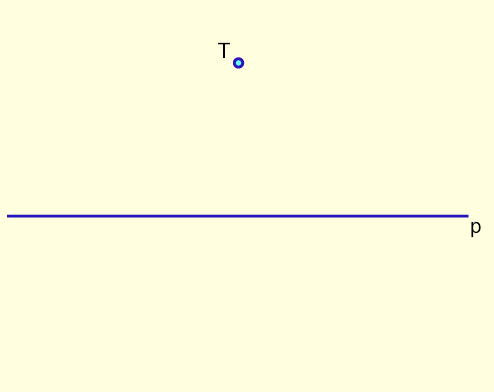
\includegraphics[width=50mm]{fig-1.png}%
		%   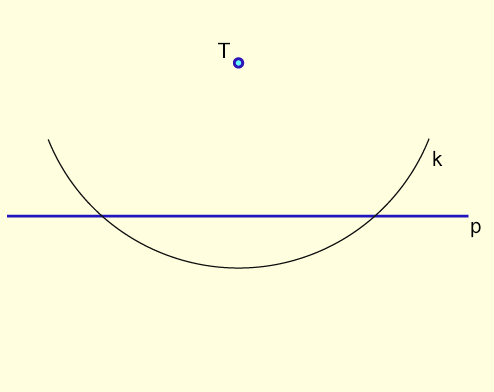
\includegraphics[width=50mm]{fig-2.png}%
		%   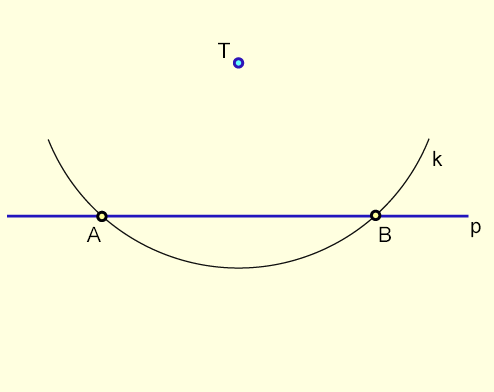
\includegraphics[width=50mm]{fig-3.png}%
		%   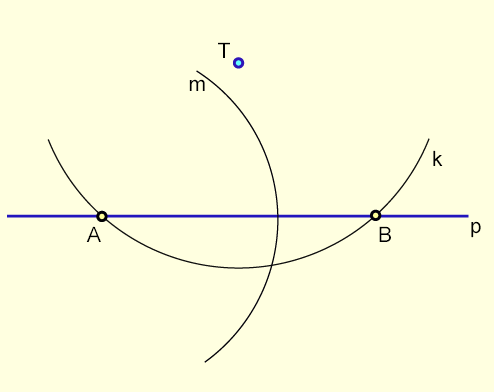
\includegraphics[width=50mm]{fig-4.png}%
		%   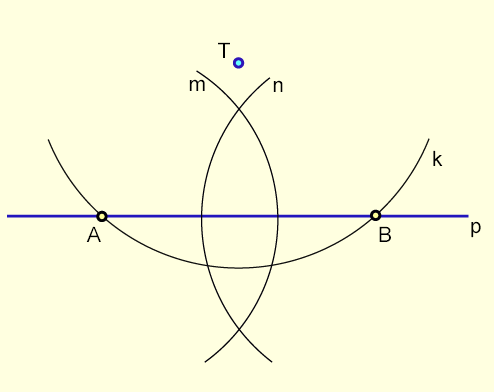
\includegraphics[width=50mm]{fig-5.png}%
		%   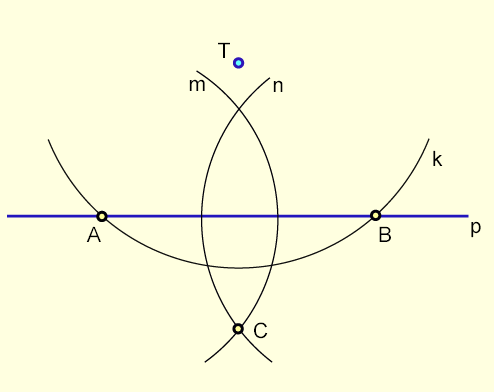
\includegraphics[width=50mm]{fig-6.png}%
		%   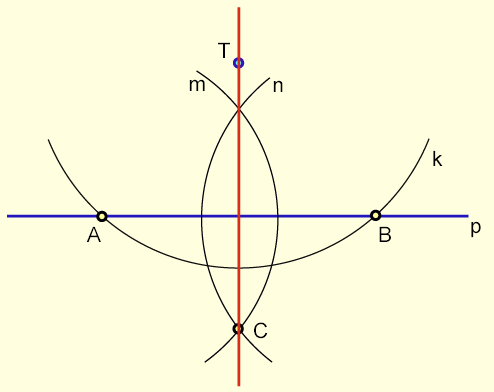
\includegraphics[width=50mm]{fig-7.png}%

\end{frame}

				% Spodnje je za nalogo 3.4.

				% % Sliko smo naredili tako, da so točke A, B, T in C vse enako oddaljene
				% % od presečišča premic; kot ATC je 45°.
				% % Vsi krožni loki imajo radij 2.
				% \tikzmath{
				% 	% Razdalja od točke T do premice p je tako 2*sin(45°).
				% 	\t = 2*sin(45);
				% 	% Razdalja začetka loka m do premice p
				% 	% oz. razdalja točke T' levo in zgoraj od točke T do premice
				% 	\tt = 2*sin(60);
				% 	% Razdalja točke T' od navpične premice skozi T
				% 	\td = \t-2*cos(60);
				% }
				% % Definicija točke T
				% \coordinate [label={[blue, above left]:$T$}] (T) at (0,{\t});
				% % Risanje točke T
				% \fill[blue] (T) circle (2pt);
				% % Premica p
				% \draw[blue, very thick] (-2,0) -- (2,0) node[right] {$p$};
				% \pause
				% % Definicija pomožne točke A' in risanje krožnega loka k, ki se začne v A'
				% \coordinate (A') at ({-\tt},{\td});
				% \draw[gray, thin] (A') arc[start angle=210, end angle=330, radius=2] node[right] {\scriptsize $k$};
				% \pause
				% % Točka A
				% \coordinate [label=below left:{\scriptsize $A$}] (A) at ({-\t},0);
				% \draw (A) circle (1.5pt);
				
				% % Naloga 3.4.1.: Narišite še točko B (skupaj z oznako)
				
				% % Naloga 3.4.2.: Definirajte točko T', v kateri se začne lok m in narišite lok m z oznako.
				% % Lok je definiran s točko, v kateri se lok začne (ne središče!), z začetnim in končnim kotom ter radijem.
				% % Koti so vedno podani enako: kot 0 je v smeri x osi in se veča v nasprotni smeri urinega kazalca.

				% % Naloga 3.4.3.: Definirajte točko T'' in narišite lok n z oznako.
				
				% % Naloga 3.4.4.: Definirajte in narišite točko C.

				% % Naloga 3.4.5.: Narišite premico skozi točki T in C.

				% Konec vsebine za nalogo 3.4.


% Naloga 4
% \begin{frame}{Graf funkcije s TikZ}
% 	\centering
% 	\begin{tikzpicture}
% 		\begin{axis}[
% 			axis lines = middle,
% 			domain = 0:10,
% 			width = 9cm,
% 			height = 8cm,
% 			xtick = {0, 1, 2, 3, 4, 5, 6, 7, 8},
% 			ytick = {0, 1, 2, 3, 4, 5, 6},
% 			ymin = -1,
% 			ymax = 7,
% 			grid = both
% 		]
% 		\end{axis}
% 	\end{tikzpicture}
% \end{frame}

% Sekcija 5 - Paket beamer in tabele
\section{Paket \texttt{beamer} in tabele}
\begin{frame}{Odkrivanje tabele po vrsticah}
	Včasih pride prav, da tabelo odkrivamo postopoma po vrsticah.
	\begin{center}
		\begin{tabular}{c|cccc}
		   Oznaka & A & B & C & D \\ \hline 
		   \pause
		   X & 1 & 2 & 3 & 4 \\ 
		   \pause
		   Y & 3 & 4 & 5 & 6 \\ 
		   \pause
		   Z & 5 & 6 & 7 & 8 
		\end{tabular}
	\end{center}
\end{frame}
 

\begin{frame}{Odkrivanje tabele po stolpcih}
	Tabelo lahko odkrivamo tudi po stolpcih, čeprav ni najlažje.

	\begin{center}
		\begin{tabular}{c|>{\onslide<2->}c<{\onslide<3->}c>{\onslide<4->}c>{\onslide<5->}c>{\onslide}}
		   Oznaka & A & B & C & D \\ \hline
		   X & 1 & 2 & 3 & 4 \\
		   Y & 3 & 4 & 5 & 6 \\
		   Z & 5 & 6 & 7 & 8
		\end{tabular}
	\end{center}
\end{frame}


% Sekcija 6 - Matematične vsebine (Zaporedja, algebra, grupe)
\section[Matematika, 2. del\\\large{Zaporedja, algebra, grupe}]{Matematika, 2. del}
\begin{frame}{Zaporedja, vrste in limite}
	\begin{enumerate}
		\item 
		Naj bo ?? absolutno konvergentna vrsta in $a_n \ne -1$.
		Dokaži, da je tudi vrsta $\sum_{n=1}^\infty \frac{a_n}{1+a_n}$
		absolutno konvergentna.

		\item
		Izračunaj limito
		??

		\item
		Za dani zaporedji preveri, ali sta konvergentni.
		% Pomagajte si s spodnjima delno pripravljenima matematičnima izrazoma:
		% a_n = \sqrt{2+\sqrt{2+\dots+\sqrt{2}}} \qquad
		% b_n = \sin(\sin(\dots(\sin 1)\dots))
		??
	\end{enumerate}
\end{frame}

\begin{frame}{Algebra}
	\begin{enumerate}
		\item
		Vektorja ??
		sta pravokotna in imata dolžino 1. Določi kot med vektorjema $\vec{a}$ in $\vec{b}$.
		\item 
		Izračunaj
		??
	\end{enumerate}
\end{frame}

\begin{frame}{Velika determinanta}
	Izračunaj naslednjo determinanto $2n \times 2n$, ki ima na neoznačenih mestih ničle.
	??
\end{frame}

\begin{frame}{Grupe}
	Naj bo
	??
	\begin{enumerate}
		\item
			Pokaži, da je $G$ podgrupa v grupi ??
			neničelnih kompleksnih števil za običajno množenje.
		\item
			Pokaži, da je $H$ podgrupa v aditivni grupi ??
			ravninskih vektorjev za običajno seštevanje po komponentah.
		\item
			Pokaži, da je preslikava $f:H\to G$, podana s pravilom
			??
			izomorfizem grup $G$ in $H$.
	\end{enumerate}
\end{frame}


\end{document}